%!TEX root = gutter+stars.tex

%%%%%%%%%%%%%
%%%%%%%%%%%%%
%%%%%%%%%%%%%
%%%%%%%%%%%%%
%%%%%%%%%%%%%
%%%%%%%%%%%%%
%%%%%%%%%%%%%
%%%%%%%%%%%%%

\chapter{Software Cartography}
\label{the chapter on codemap}

\infobox
	{Code orientation in general}
	{Local codebase and possibly history of a system}
	{Spatial (established through lexical and structural information)}
	{Visual analytics of a cartographic visualization}



\asteriskasteriskasterisk

Current tool support for code orientation by spatial clues is \adhoc at best, most striking is the lack of spatial on-screen representations of source code. Without such a representation developers are barely able to draw on the strong spatial capability of the human brain. 

We provide a cartographic on-screen visualization such that developers can start using spatial clues for code orientation. Since software has no inherent spatial structure we use lexical and structural information found in the source code to establish a spatial layout of the local code base. The created \emph{software maps} are stable over time and can be shared among members of a team to establish a common mental model of the system. 
%
We implemented our approach in a prototype, evaluated it in a user study, and found that it is most helpful for spatially exploring search results and call hierarchies.

Software visualization can provide a concise overview of a complex software system. Unfortunately, since software has no physical shape, there is no ``natural'' mapping of software to a two-dimensional space. As a consequence most visualizations tend to use a layout in which position and distance have no meaning, and consequently layout typically diverges from one visualization to another. We propose an approach to consistent layout for software visualization, called \emSOCA, in which the position of a software artifact reflects its \emph{vocabulary}, and distance corresponds to similarity of vocabulary. We use a vector-space model to map software artifacts to a vector space, and then a combination of the Isomap algorithm \cite{Tene00a} and Multidimensional Scaling \cite{Borg05a} is used to map this vector space down to two dimensions. The resulting consistent layout allows us to develop a variety of thematic \emph{software maps} that express very different aspects of software while making it easy to compare them. The approach is especially suitable for comparing views of evolving software, since the vocabulary of software artifacts tends to be stable over time. We present a prototype implementation of \SOCA, and illustrate its use with practical examples from numerous open source case studies.

\section{Spatial Representation of Software}

Software visualization offers an attractive means to abstract from the complexity of large software systems. A single graphic can convey a great deal of information about various aspects of a complex software system, such as its structure, the degree of coupling and cohesion, growth patterns, defect rates, and so on \cite{Dieh07a,Kien07a,Reis05a,Stor05a}. Unfortunately, the great wealth of different visualizations that have been developed to abstract away from the complexity of software has led to yet another source of complexity: it is hard to compare different visualizations of the same software system and correlate the information they present.

We can contrast this situation with that of conventional thematic maps found in an atlas.
Different phenomena, ranging from population density to industry sectors, birth rate, or even flow of trade, are all displayed and expressed using \emph{the same consistent layout}.
It easy to correlate different kinds of information concerning the same geographical entities because they are generally presented using the same kind of layout.
This is possible because (i) there is a natural mapping of position and distance information to a two-dimensional layout\footnote{Even if we consider that the Earth is not flat on a global scale, there is still a natural mapping of position and distance to a two-dimensional layout; see the many types of cartographic projections (\eg the Mercator projection) used during centuries to do that. In fact, this is true for a large class of manifolds.}, and (ii) because by convention North is normally considered to be on the top.\footnote{The orientation of modern world maps, that is North on the top, has not always been the prevailing convention. On traditional Muslim world maps, for example, South used to be in the top. Hence, if Europe would have fallen to the Ottomans at the Battle of Vienna in 1683, all our maps might be drawn upside down by now \cite{Hite99a}.}

Software artifacts, on the other hand, have no natural layout since they have no physical location.
Distance and orientation also have no obvious meaning for software.
It is presumably for this reason that there are so many different and incomparable ways of visualizing software.
A cursory survey of recent \textsc{Softvis} and \textsc{Vissoft} publications shows that the majority of the presented visualizations feature arbitrary layout, the most common being based on alphabetical order and \emph{arbitrary hash-key order}.
(Hash-key order is what we get in most programming languages when iterating over the elements of a Set or Dictionary collection.)

Robert DeLine's work on software navigation \cite{Deli05b,Deli06a} closely relates to \SOCA. His work is based on the observation that developers are consistently lost in code \cite{Deli05a} and that using textual landmarks only places a large burden on cognitive memory. He concludes the need for new visualization techniques that allow developers to use their spatial memory while navigating source code.

DeLine proposes four desiderata \cite{Deli05b} that should be satisfied by spatial software navigation: 1)~the display should show the entire program and be continuous, 2)~the display should contain visual landmarks such that developers can find parts of the program perceptually rather than relying on names, 3)~the display should remain visually stable during navigation [and evolution], and 4)~the display should be capable of showing global program information overlays other than navigation. An ad-hoc algorithm that satisfies the first and fourth properties is presented in the same work. 

Our work satisfies all above desiderata, and completes them with a fifth desideratum that visual distance should have a meaningful interpretation. The scope of \SOCA is broader than just navigation, it is also intended for reverse engineering and code comprehension in general. We can thus generalize the five desiderata for spatial representation of software as follows:

\begin{enumerate}
\item The visualization should show the entire program and be continuous.
\item The visualization should contain visualization landmarks that allow the developers to find parts of the system perceptually, rather than relying on name or other lexical clues. 
\item The visualization should remain visually stable as the system evolves. 
\item The visualization should should be capable of showing global information overlays.
\item On the visualization, distance should have a meaningful interpretation. 
\end{enumerate}

% ===================================================================================
\section{Software Cartography}
\label{sec:techniques}

Consistent layout for software would make it easier to compare visualizations of different kinds of information. But what should be the basis for positioning representations of software artifacts within a ``cartographic'' software map?
What we need is a semantically meaningful notion of position and distance for software artifacts, a spatial representation of software in a multi-dimensional space, which can then be mapped to consistent layout on the 2-dimensional visualization plane.

We propose to use \emph{vocabulary} as the most natural analogue of physical position for software artifacts, and to map these positions to a two-dimensional space as a way to achieve consistent layout for software maps. Distance between software artifacts then corresponds to distance in their vocabulary. We use a combination of the Isomap algorithm \cite{Tene00a} and Multidimensional Scaling \cite{Borg05a} to projection the high-dimensional vector space model onto the two-dimensional visualization pane. Finally we use cartographic techniques (such as digital elevation, hill-shading and contour lines) to generate a landscape representing the frequency of topics. We call our approach \emSOCA, and call a series of visualizations \emph{Software Maps}, when they all use the same consistent layout created by our approach. 

Why should we adopt vocabulary as distance metric, and not some structural property?
First of all, vocabulary can effectively \emph{abstract} away from the technical details of source code \cite{Kuhn07a} by capturing the key domain concepts of source code. Software entities with similar vocabulary are conceptually and topically close. Lexical similarity has proven useful to detect high-level clones \cite{Marc01a} and cross-cutting concerns \cite{Pali08a} in software. Furthermore, it is known that over time vocabulary tends to be more stable than the structure of software \cite{Anto07a}, and tends to grow rather than to change \cite{Vasa07b}. Although refactorings may cause functionality to be renamed or moved, the overall vocabulary tends not to change, except as a side-effect of growth. This suggests that vocabulary will be relatively \emph{stable} in the face of change, except where significant growth occurs. As a consequence, vocabulary not only offers an intuitive notion of position that can be used to provide a consistent layout for different kinds of thematic maps, but it also provides a robust and consistent layout for mapping an evolving system. System growth can be clearly positioned with respect to old and more stable parts of the same system.

\begin{figure}
\begin{center}
  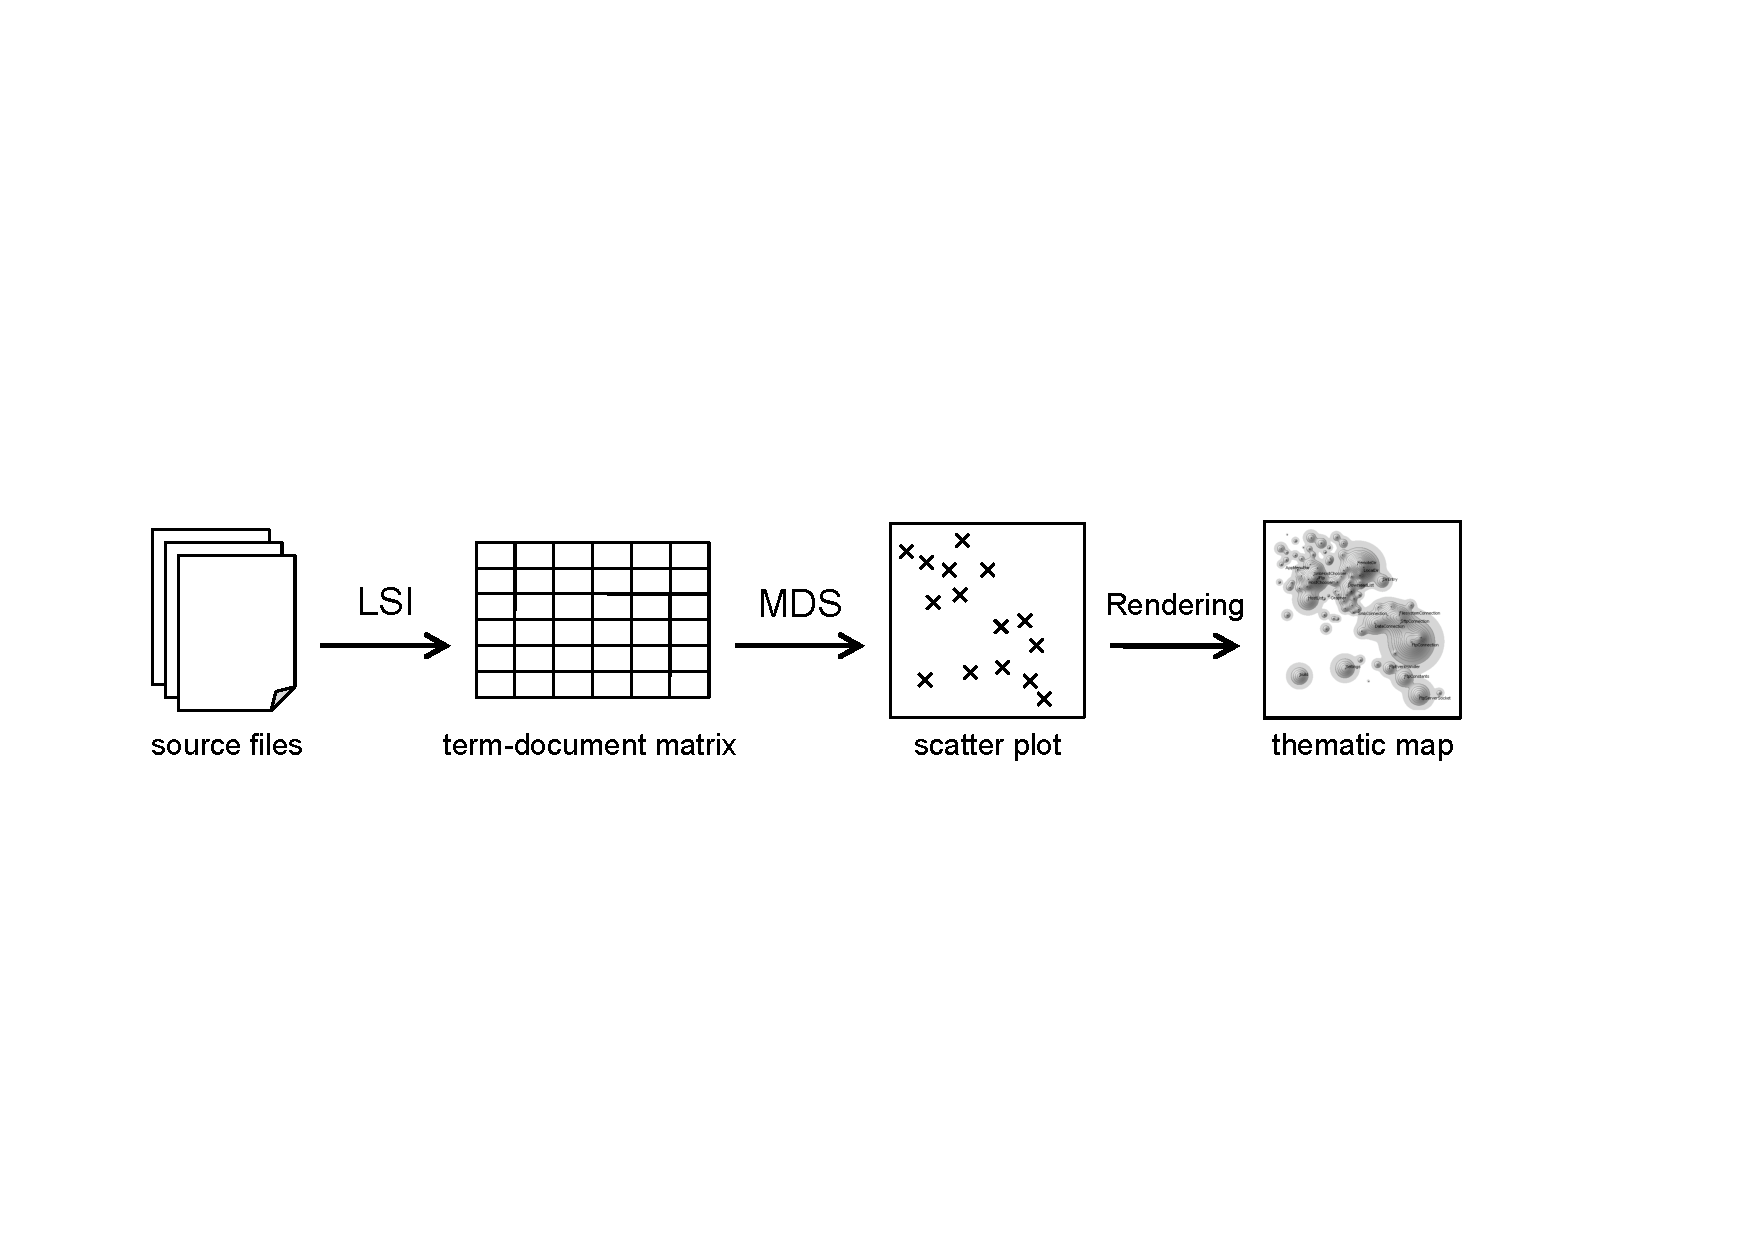
\includegraphics[width=\linewidth]{fig/codemap-pipeline}
\end{center}
    \caption{\SOCA in a nutshell: left) the raw text of source files are parsed and indexed, center) the high-dimensional term-document-matrix is mapped down to two dimensions using \MDS and Isomap, and right) cartographic visualization techniques are used to render the final map.}
    \label{fig:soca}
\end{figure}

In the following we present the techniques that are used to achieve a consistent layout for software maps.
The general approach of \SOCA, as illustrated in \autoref{fig:soca}, is as follows:
%\begin{enumerate}
%\item We parse the vocabulary of source files into term-frequency histograms. All text found in raw source code is taken into account, including not only identifiers but also comments and literals.
%\item We use a combination of the Isomap algorithm \cite{Tene00a} and Multidimensional Scaling \cite{Borg05a} to map the term-frequency histograms onto the 2D visualization pane. This preserves the lexical co-relation of source files as well as possible.
%\item We use cartographic visualization techniques to render an aesthetically appealing landscape.
%\end{enumerate}

%Possible applications of \SOCA in the software development process are, \dots
%\begin{itemize}
%\item \dots to navigate within a software system, be it for development or analysis.
%\item \dots to relate different metrics to each other, \eg search results and bug prediction.
%\item \dots to stay in touch with other developers of your team, by showing open files of other developers.
%\item \dots to understand a system�s domain upon first contact.
%\item \dots to explore a system during reverse engineering.
%\end{itemize}

\begin{description}

\item[Information Retrieval] We parse the vocabulary of source files into term-frequency histograms. All text found in raw source code is taken into account, including not only identifiers but also comments and literals.

\item[2-Dimensional Embedding]
A metric distance is used to compute the pair-wise dissimilarity of software artifacts (typically source code files). A combination of the Isomap algorithm \cite{Tene00a} and Multidimensional Scaling \cite{Borg05a} is used to embed all software artifacts on the visualization pane. Other than with Lexical Clustering, as presented in \autoref{the chapter on hapax}, we do not apply Latent Semantic Indexing as it has been found to have little impact on the final embedding, if at all. The application of Isomap is an improvement of the embedding in order to assist MDS with the global layout. The final embedding minimizes the error between the dissimilarity values and the visual distances.

Early prototypes of \Codemap used a distance metric that was based on lexical similarity only. However, our user study revealed that developers tend to interpret visual distance as a measure of structural dependencies, even though they were aware of the underlying lexical implementation. Based on this observation, we developed an improved distance metric that takes both lexical similarity and structural distance (based on the ``Law of Demeter'' \cite{Lieb88a}) into account. 

\item[Digital Elevation Model] In the next step, a digital elevation model is created. Each software artifact contributes a Gaussian shaped basis function to the elevation model according to its KLOC size. The contributions of all software artifacts are summed up and normalized. 

%Using KLOC leads to an elevation model where large classes dominate the codemap. Observations from our user study, presented on the next chapter, indicate that this might be misleading since developers tend to interpret size as a measure of impact. Based on this observation, we implemented a set of different impact metrics~\cite{Lanz06a} and plan to evaluate them in a fresh user study.

\item[Cartographic rendering] In the final step, hill-shading is used to render the landscape of the software map. Please refer to previous work for full details~\cite{Kuhn08b}. Metrics and markers are rendered in transparent layers on top of the landscape. Users can toggle separate layer on/off and thus customize the codemap display to their needs.

\end{description}


\noindent We implemented a prototype of our approach, \CODEMAP, which is available as an open source project. \CODEMAP was originally programmed in Smalltalk, in the mean time development has been moved to Java. \CODEMAP is available as an Eclipse plug-in\footnote{\url{http://scg.unibe.ch/codemap}}.

%\subsection{Iterative Online \SOCA}
%
%In our previous work we presented a technique to create software maps given either a single release, or all releases of a system at once \cite{Kuhn08b}. In this chapter we propose an improved algorithm for incremental software maps that update as new changes appear. 
%
%The offline scenario processes all releases in one pass. 
%
%\begin{itemize}
%
%\item The offline variation processes all releases of a software system at once, up to and until the projection step. Only then the location data is grouped by release, and an separate map for each release is rendered. That is both lexical similarity as well as position on the map anticipate all future evolvements from the first map on, since indexing and scaling take information of all releases into account. This scenario requires that information about all releases is available, which is given when performing post-mortem analysis of an existing system.
%
%\item The online variation processes the input release by release (or, when integrated into a development environment, even change by change). For each release, the current source as well as information carried over from the previous \SOCA computation are used. In a first step, the source files of the current release and of previous releases are parsed into a term-document matrix. This allows removed and added topics to be detected. In the next step, the lexical similarity of all current source files is fed into the projection step---together with the positions on the previous map as starting points, thus leading to more visual stability.
%
%\end{itemize}
%
%Given a series of releases both variations yield a visually stable sequence of maps. Maps generated with the iterative algorithm are less stable over time compared to the post-mortem approach. The instability of the iterative approach decreases over time, since the amount of accumulated historical data increases with each release. In general, the iterative algorithm is less sensitive to the addition or removal of entire topics between releases, such changes are better observed by performing post-mortem analysis. Please refer to the evaluation in Section~\ref{sec:hausdorff} for more details.

%For example, the JUnit case-study in section  (Hausdorff distance $0.25 \pm 0.11$ versus $0.10 \pm 0.14$).

% -----------------------------------------------------------------------------------
\subsection{Lexical Similarity between Source Files}
\label{sec:lsi}

As motivated in the introduction, the distance between software entities on the map is based on the lexical similarity of source files. Lexical similarity is an Information Retrieval (IR) technique based on the vocabulary of text files. Formally, lexical similarity is defined as the cosine between the term frequency vectors of two text documents. That is, the more terms (\ie identifier names and operators, but also words in comments) two source files share, the closer they are on the map. 

First, the raw source files are split into terms. Then a matrix is created, which lists for each document the occurrences of terms. Typically, the vocabulary of source code consists of 500--20'000 terms. In fact, studies have shown that the relation between term count and software size follows a power law \cite{Zhan08a}. For this work, we consider all text found in raw source files as terms. This includes class names, methods names, parameter names, local variables names, names of invoked methods, but also words found in comments and literal values. Identifiers are further preprocessed by splitting up the camel-case name convention which is predominantly used in Java source code. Note that since our approach is based on raw text, any programming language that uses textual source files might  be processed.

% -----------------------------------------------------------------------------------
\subsection{Multi-dimensional Scaling}

In order to visualize the lexical similarity between software entities, we must find a mapping that places source files (or classes, or packages, depending in our definition of a document) on the visualization pane. The placement should reflect the lexical similarity between source files.

We use a combination of the Isomap algorithm \cite{Tene00a} and Multidimensional Scaling \cite{Borg05a} in order to map from the previously established multi-dimensional term-document matrix down to two dimensions.
 \MDS tries to minimize a stress function while iteratively placing elements into a low-level space. \MDS yields the best approximation of a vector space's orientation, \ie it preserves the distance relation between elements as best as possible. This is good for data exploration problems.

\newlength{\figwidth}
\begin{figure}
\begin{center}
  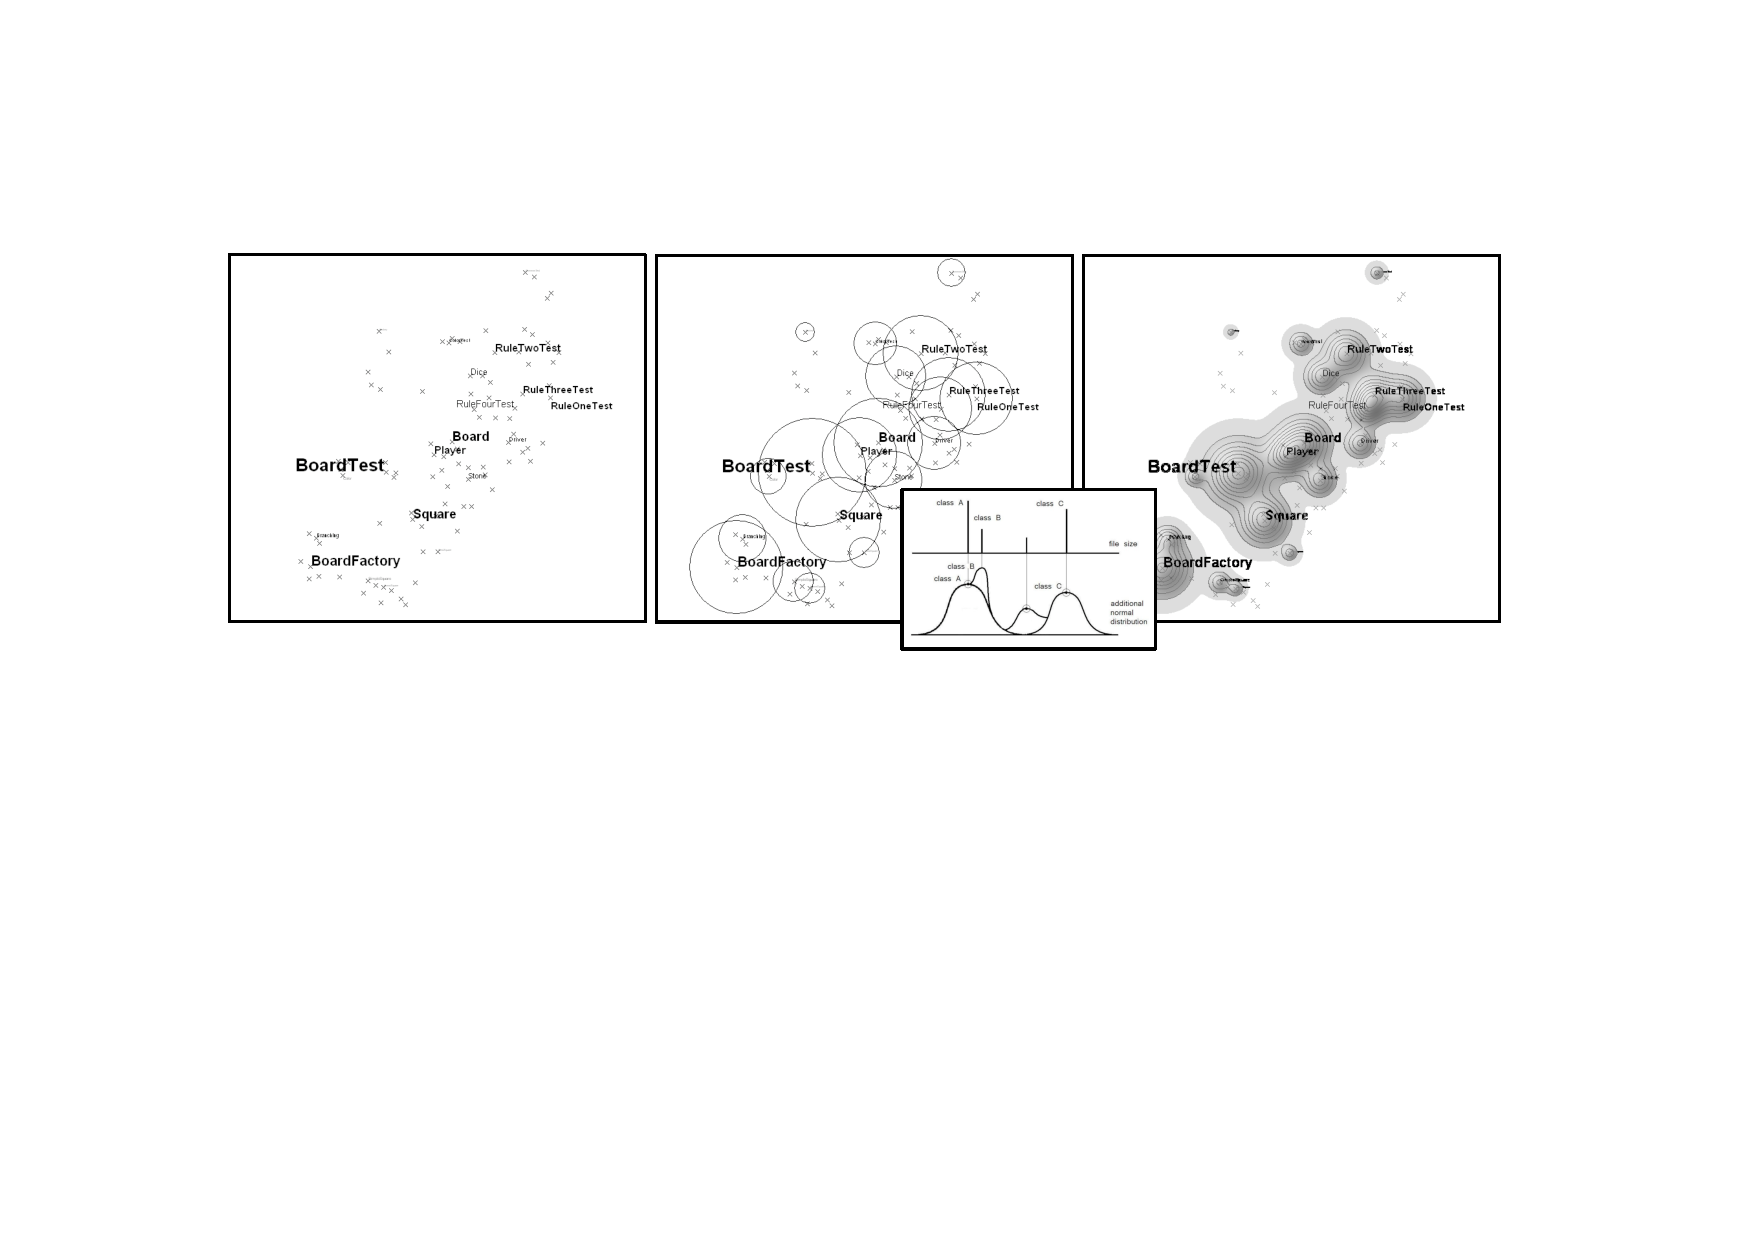
\includegraphics[width=\linewidth]{fig/codemap-pipeline-too.pdf}
\end{center}
    \caption{Construction steps: left) the projection step placement of files on the visualization pane, middle) circles around each file's location, based on class size in KLOC, right) digital elevation model with hill-shading and contour lines. Sidebox on digital elevation model) each file contributes a Gaussian shaped basis function to the elevation model according to its KLOC size. The contributions of all files are summed up to a digital elevation model.}
    \label{fig:steps}
\end{figure}

% -----------------------------------------------------------------------------------
\subsection{Cartographic Visualization Techniques}

Eventually, we use hill-shading \cite{Burr98a} to render an aesthetically appealing landscape. \autoref{fig:steps} illustrates the final rendering steps of \SOCA. On the final map, each source file is rendered as a hill whose height corresponds to the entity's KLOC size.

Hill-shading uses a digital elevation model (DEM) to render the illumination of a landscape. The digital elevation model is a two-dimensional scalar field. Each each entity contributes a Gaussian shaped basis function to the elevation model. To avoid that closely located entities occlude each other, the contributions of all files are summed up as shown in \figref{steps}. 

A map without labels is of little use. On a software map, all entities are labeled with their name (class or file name). Labeling is a non-trivial problem, as an algorithm is needed to ensure that labels do not overlap. Also labels should not obscure important landmarks. Most labeling approaches are semi-automatic and need manual adjustment, an optimal labeling algorithm does not exist \cite{Sloc05a}. 

For locations that are near to each other it is difficult to place the labels so that they do not overlap and hide each other. For software maps it is even harder due to often long class names and clusters of closely related classes. This work uses a greedy brute-force algorithm for labeling. Labels are placed in order of hill size, \ie the name of the largest file is placed first, and so on. If a to-be placed label would overlap with an already placed label, the to-be placed label is omitted. Thus, the labels of smaller files are typically omitted in favor of the labels of larger files.

% =============================================================================
\section{On the Choice of Vocabulary}
\label{sec:onvocabulary}

The decision to use a distance based on lexical similarity does, indeed, create a distribution of distances that should not change a lot in time. This is because programmers will not use a completely new set of lexical tokens in each new version of the software. In fact, it has been shown that over time vocabulary tends to be more stable than the structure of software \cite{Anto07a}. However, this also will create software maps that naturally only can show how items are similar from a lexical point of view.

The map layout as presented in this work can, of course, be used to see how items are related from the point of view of some other distance metric, such as considering structural similarity, similarity with regard to a complexity or testability metric. In that case, the distance may vary a lot over time during the evolution of a product, and this will create unstable layouts. The focus of this work, however, is the creation of maps that help programmers to establish a stable mental model of their software system under work. In any case, if maps  based on other metrics are ever to be used in conjunction with vocabulary-based \SOCA maps, we strongly recommend to visually distinguish them by using another rendering scheme. This helps to reduce the likeliness that programmers confuse the spatial layout of these other maps, with the mental model acquired through the use of \SOCA maps. 

As mentioned above, \SOCA is vocabulary-based because vocabulary can effectively \emph{abstract} away from the technical details of source code \cite{Kuhn07a} by capturing the key domain concepts of source code. The assumption is that software entities with similar vocabulary are conceptually and topically close. Consider, for example, programming languages and software where methods may be overloaded. Even though overloaded methods differ in their implementation strategy, they will typically implement the same concept using the same vocabulary. In fact, lexical similarity has proven useful to detect high-level clones \cite{Marc01a} and cross-cutting concerns \cite{Pali08a} in software.  

Although refactorings may cause functionality to be renamed or moved, the overall vocabulary tends not to change, except as a side-effect of growth \cite{Zhan08a,Vasa07b}. Consider the example of a rename refactoring. Two effects may occur. 
In the first case, all occurrences of a symbol are replaced with new symbol. This will not affect the map, since lexical similarity is based on statistical analysis only. Replacing all occurrences of one term with a new term is, from the point of these IR technologies, a null operation. In the second case, some occurrences of a symbol are replaced with another symbol which is already used. This will indeed affect the layout of the map. Given that the new name was well chosen by the programmer, the new layout will constitute a better representation of the system. On the other hand, if the new name is a bad choice, the new layout will be flawed. However, what constitutes bad naming is not merely a matter of taste. Approaches that combine vocabulary with structural information can indeed assess the quality of naming. Please refer to H\o{}st's recent work on debugging method names for further reading \cite{Hoes09a}.

Not considered in the present work is the relative weight of different lexical tokens. For example, it seems reasonable to weight local identifiers differently than identifiers in top-level namespaces. Also, one may treat names coming from library functions different from the ones coming from the actual user code. Given the absence of evaluation benchmarks, we decided to use equal weighting for all lexical tokens. Also, preliminary experiments with different weighting schemes indicate that relative weights below boost level, \ie below a factor of 10, do often not significantly affect the overall layout.

% =============================================================================
\section{Example: the Story of Ludo}
\label{sec:casestudy}

In this section we present an example of \SOCA. Figure~\ref{fig:ludo} shows the complete history of the Ludo system, consisting of four iterations. Ludo is used in a first year programming course to teach iterative development. The 4th iteration is the largest with 30 classes and a total size of 3-4 KLOC. We selected Ludo because in each iteration, a crucial part of the final system is added. 

\begin{itemize}

\item The first map (\autoref{fig:ludo}, leftmost) shows the initial prototype. This iteration implements the board as a linked list of squares. Most classes are located in the south-western quadrant. The remaining space is occupied by ocean, nothing else having been implemented so far.

\item In the second iteration (\autoref{fig:ludo}, second to the left) the board class is extended with a factory class. In order to support players and stones, a few new classes and tests for future game rules are added. On the new map the test classes are positioned in the north-eastern quadrant, opposite to the other classes. This indicates that the newly added test classes implement a novel feature (\ie testing of the game's ``business rules'') and are thus not related to the factory's domain of board initialization. 

\item During the third iteration (\autoref{fig:ludo}, second to the right) the actual game rules are implemented. Most rules are implemented in the {\tt Square} and {\tt Ludo} class, thus their mountain rises. In the south-west, we can notice that, although the {\tt BoardFactory} has been renamed to {\tt LudoFactory}, its position on the map has not changed considerably. 

\item The fourth map (\autoref{fig:ludo}, rightmost) shows the last iteration. A user interface and a printer class have been added. Since both of them depend on most previous parts of the application they are located in the middle of the map. Since the new UI classes use vocabulary from all parts of the system, the islands are joined into a continent.

\end{itemize}

The layout of elements remains stable over all four iterations.  For example, {\tt Board/LudoFactory} is on all four views located in the south-western quadrant.

\begin{figure*}
  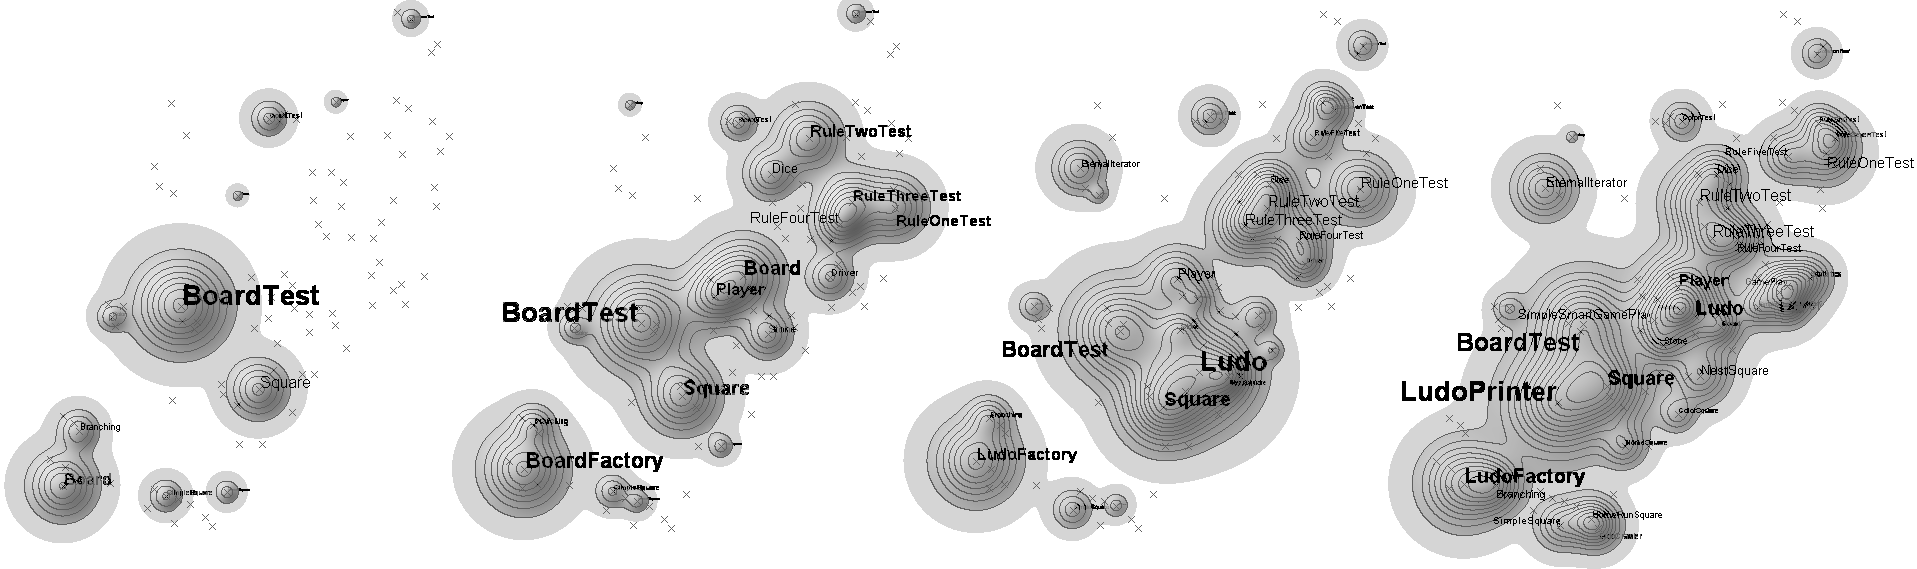
\includegraphics[width=\linewidth]{fig/chronia-ludo-history}
  \caption{From left to right: each map shows four iterations of the same software system. As all four views use the same layout, a user can build up a mental model of the system's spatial structure. For example, {\tt Board/LudoFactory} is on all four views located in the south-western quadrant. See also Figure~5 and 6 for more views of this system.}
  \label{fig:ludo}
\end{figure*}

\section{Discussion}

\SOCA, as presented in this chapter, is a spatial representation of software. Our approach visualizes software entities using a consistent layout. Software maps present the entire program and are continuous. Software maps contain visual landmarks that allow developers to find parts of the system perceptually rather then relying on conceptual cues, \eg names. Since all software maps of a system use the same layout, maps with thematic overlays can be compared to each other.

The layout of software maps is based on the lexical similarity of software entities. Our algorithm uses a vector-space model to position software entities in an multi-dimensional space, and a combination of the Isomap algorithm \cite{Tene00a} and Multidimensional Scaling \cite{Borg05a} to map these positions on a two-dimensional display. Software maps can be generated to depict evolution of a software system over time. We evaluated the visual stability of iteratively generated maps considering four open source case studies.

In spite of the aesthetic appeal of hill shading and contour lines, the main contribution of this chapter is not the cartographic look of software maps. The main contribution of \SOCA is (i) that cartographic position reflects topical distance of software entities, and (ii) that consistent layout allows different software maps to be easily compared.
In this way, software maps reflect world maps in an atlas that exploit the same consistent layout to depict various kinds of thematic information about geographical sites.

Software maps at present are largely static. In a more interactive environment the user can ``zoom and pan'' through the landscape to see features in closer detail, or navigate to other views of the software. The \textsc{CodeCanvas} prototype by Deline and Rowan offers this feature \cite{Deli10a}. All source code is put on a large zoomable canvas and developers zoom and pan around on this canvas as they work on the system. Depending on the zoom level of the canvas a different semantic view of the system is shown. For example, as the canvas is zoomed out the source code fades off and labels with colored icons appear instead to mark the signature of methods.

Selectively displaying features would make the environment more attractive for navigation. Instead of generating all the labels and thematic widgets up-front, users can annotate the map, adding comments and waymarks as they perform their tasks. The \textsc{CodeBubbles} prototype by Bragdon and Reiss offers this feature \cite{Brag10b}. Instead of offering one global representation, a custom spatial layout of separate method bodies is unfolded as the developer works on the code. For each working context, \ie task, a new view is generated. They offer specialized views for debugging contexts, including a differential debugging mode. They are evaluating their prototype in an ongoing series of user studies, on the first of which is being reported in their current publications \cite{Brag10a,Brag10b}.

Orientation and layout are presently consistent for a single project only. The usefulness of conventions for establishing consistent layout and orientation (\ie ``testing'' is North-East) that will work across multiple projects, possibly within a reasonably well-defined domain, is an open issue. However, given the findings of the user study presented in the next chapter, we consider it to be more worthwhile to invest in customizable layouts rather than predefined global layouts. 

%Even though, generating a map of \eg all available open-source projects might be worthwhile on its own accord.


%%%%%%%%%%%%%
%%%%%%%%%%%%%
%%%%%%%%%%%%%
%%%%%%%%%%%%%
%%%%%%%%%%%%%
%%%%%%%%%%%%%
%%%%%%%%%%%%%
%%%%%%%%%%%%%

\chapter{User Study on Software Cartography}
\label{the chapter on the codemap user study}

Software visualization can be of great use for understanding and exploring a software system in an intuitive manner. Spatial representation of software is a promising approach of increasing interest. However, little is known about how developers interact with spatial visualizations that are embedded in the IDE. In this chapter, we present a pilot study that explores the use of \SOCA for program comprehension of an unknown system. We investigated whether developers establish a spatial memory of the system, whether clustering by topic offers a sound base layout, and how developers interact with maps. We report our results in the form of observations, hypotheses, and implications. Key findings are a) that developers made good use of the map to inspect search results and call graphs, and b) that developers found the base layout surprising and often confusing. We conclude with concrete advice for the design of embedded software maps.

In the past decade the software visualization community has developed a rich wealth of visualization approaches~\cite{Dieh07a} and provided evidence of their usefulness for expert tasks, such as reverse engineering, release management or dynamic analysis (\eg \cite{Tele08b,Pauw08a,Reis05b,Orso03a}). Typically, these visualization approaches had been implemented in interactive tools \cite{Sens08a}. However most of these tools are stand-alone prototypes that have never been integrated in an IDE (integrated development environment). Little is thus known about the benefits of software visualization for the ``end users'' in software engineering, that is for everyday programmers. What is lacking is how these techniques support the day to day activities of software developers \cite{Stor05a}. 

In this chapter, we report on a pilot study of a spatial software visualization that is embedded in the IDE. The spatial visualization is based on the \SOCA approach that has been presented and introduced in previous work \cite{Kuhn08a,Kuhn10b,Erni10a}. Spatial representation of software is a promising research field of increasing interest \cite{Wett08a,Deli10a,Brag10b,Stei10a,Mart08a,Noac05a}, however the respective tools are either not tightly integrated in an IDE or have not yet been evaluated in a user study. Spatial representation of software is supposed to support developers in establishing a long term, spatial memory of the software system. Developers may use spatial memory to recall the location of software artifacts, and to put thematic map overlays in relation with each other \cite{Kuhn10b}.

%\ewe{Maybe comment somewhere that the level of integration may vary. Distant integration would be the case of the visualization being available within the IDE, but remain rather an supplementary tools. Tight integration implies that the map reacts to other events in the IDE, e.g. file close, etc. or at least stays sync'ed with the project}

The scenario of our user study is first contact with an unknown closed-source system. Our main question was whether and how developers make use of the embedded visualization and if our initial assumptions made when designing the visualization (as for example the choice of lexical similarity as the map's base layout, see \autoref{sec:onvocabulary}) are based on a valid model of developer needs. Participants had 90 minutes to solve 5 exploratory tasks and to fix one bug report. We used the think-aloud protocol and recorded the voices of the participants together with a screen capture of their IDE interactions. We took manual notes of IDE interaction sequences and annotated the sequences with the recorded think-aloud transcripts. 

Results are mixed\,---\,some support and some challenge our assumptions on how developers would use the embedded visualization. Participants found the map most useful to explore search results and call graphs, but only rarely used the map for direct navigation contrary to our expectations.
%It became quickly apparent that we should revise our initial assumption that lexical similarity is a valid basis for the cartographic layout. Participants interpreted visual distance as a measure of structural dependencies---even though they were aware of the underlying lexical implementation.

% ===================================================================================
\section{The \CODEMAP Prototype}
\label{sec:tasks}

\SOCA uses a spatial visualization of software systems to provide software development teams with a stable and shared mental model. The basic idea of cartographic visualization is to apply thematic cartography~\cite{Sloc05a} to software visualization. That is, to show thematic overlays on top of a stable, spatial base layout. Features on a thematic map are either point-based, arrow-based or continuous. For software this could be the dispersion of design flaws as visualized using icons; a call graph  is visualized as a flow map (as illustrated on \autoref{fig:awesome}); and test coverage is visualized as a choropleth map, \ie a heat map. 

\SOCA is most useful when it supports as many development tasks with spatial location awareness as possible. We therefore integrated our prototype into the Eclipse IDE so that a map of the software system may always be present. This helps developers to correlate as many development tasks as possible with their spatial location.

At the moment, the \Codemap plug-in for \eclipse supports the following tasks:\footnote{\url{http://scg.unibe.ch/codemap}}

\begin{itemize}
\item Navigation within a software system, be it for development or analysis. \Codemap is integrated with the package explorer and editor of \eclipse. The selection in the package explorer and the selection on the map are linked. Open files are marked with an icon on the map. Double clicking on the map opens the closest file in the editor. When using heat map mode, recently visited classes are highlighted on the map.

\item Comparing software metrics to each other, \eg to compare bug density with code coverage. The map displays search results, compiler errors, and (given the Eclemma plug-in is installed) test coverage information. More information can be added through a plug-in extension point.

\item Social awareness of collaboration in the development team. \Codemap can connect two or more \eclipse instances to show open files of other developers. Colored icons are used to show the currently open files of all developers. The icons are updated in real time.

\item Understand a software system's domain. The layout of \Codemap is based on clustering software by topic~\cite{Kuhn07a}, as it has been shown that, over time, the lexicon of source code is more stable than its structure~\cite{Anto07a}. Labels on the map are not limited to class names, but include automatically retrieved keywords and topics.


\item Exploring a system during reverse engineering. \Codemap is integrated with \eclipse's structural navigation features, such as search for callers, implementers, and references. Arrows are shown for search results. We apply the \textsc{Flow Map} algorithm \cite{Phan05a} to  avoid visual clutter by merging parallel arrow edges. \autoref{fig:awesome} shows the result of searching for calls to the {\tt \#getSettingOrDefault} method in the {\tt MenuAction} class.
\end{itemize}

\begin{figure}
\begin{center}
  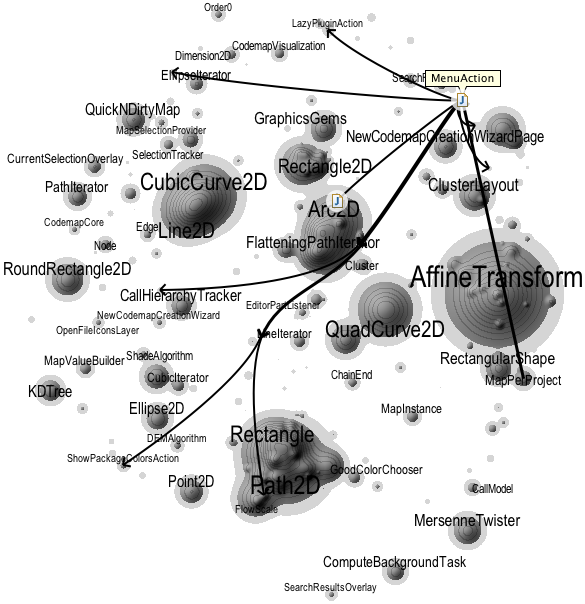
\includegraphics[width=0.7\linewidth]{fig/codemap-example}
\end{center}
    \caption{\emph{Thematic codemap of a software system. Here the \Codemap tool itself is shown. Arrow edges show incoming calls to the {\tt \#getSettingOrDefault} method in the {\tt MenuAction} class, which is currently active in the editor and thus labeled with a tool-tip.}}
    \label{fig:awesome}
\end{figure}

% ===================================================================================
\section{Methodology}
\label{sec:method}

We evaluated our approach in a pilot study with professional developers and students. The scenario investigated by the experiment is first contact with an unknown software system. Participants have 90 minutes to solve 5 program comprehension tasks and to fix one bug report. After the experiment, participants are asked to sketch their mental map of the system. 

Our goal for the present pilot study was to learn about the usability of \Codemap for program comprehension. We have been seeking to answer several questions. 
How can we support developers in establishing a spatial memory of software systems? How do we best support the developers spatial memory using software visualization? How to best embed spatial software visualization in the IDE? When provided with spatial representation of search results and call graphs, how do developers make use of them?  

Not covered in this study, and thus open for future user studies, are the shared team awareness and long term memory claims of the \SOCA approach \cite{Kuhn10b}.

%\AK{More to come here.}
%\todo{Need more background about the design rational of the study, about what we cover from our claims (ie that codemap helps to explore unknown software and that codemap helps to build up a spatial model) and which we do not cover (that the model is stable over months or years, that multiple team members share the same model, etc) and why we've chosen to cover those. Also tell why we do an exploratory study instead of going with the herd and doing one of those controlled experiments ... Cite interview with Andy Ko ftw! Also tell here that we would address other stake holders, like managers and architects that are supposed to share the same long term, spatial memory.}
%\on{this one? \url{http://doi.ieeecomputersociety.org/10.1109/MS.2009.122} -- does not seem right}
%
%
%\ewe{What I do lack so far is a clear explanation of your assumption about the map's role: (1) do you expect the map to become a central tool in development, or an auxiliary help (2) what's your position regarding "there is more than one way to do one thing", and how do you deal with it in the study. E.g. a dev uses the map to locate search result another not. Is it positive or negative? (3) what was the rationale to design these feature in the map, e.g. we thought that   synchronizing the map with the open files would benefit development because xzy. Then you can validate or invalidate each hypothesis}

\subsection{Design of the Study}

The study consists of six programming tasks. The training task introduced the participants to the \Codemap plug-in. The first five tasks were program comprehension tasks, starting with general questions and then going into more and more detailed questions. Eventually, the last task was to fix an actual bug in the system. Participants were asked to use the map whenever they saw fit, but otherwise they were free to use any other feature of Eclipse they wanted.

\paragraph{Task 1, Domain and Collaborators} \emph{``Find the purpose of the given application and identify the main collaborators. Explore the system, determine its domain, and fulfil the following tasks: a) describe the domain, b) list the main collaborators, c) draw a simple collaboration diagram, d) identify the main feature of the application.''}

\paragraph{Task 2, Technologies} \emph{``In this task we are interested in the technologies used in the application. List the main technologies, such as for example Ajax, XML, or unit testing.''}

\paragraph{Task 3, Architecture}  \emph{``In this task we are going to take a look at the architecture of the application. Reverse engineer the architecture by answering the following questions: a) which architectural paradigm is used (as for example pipes and filters, layers, big ball of mud, etc)? b) what are the main architectural components? c) how are those components related to one another? d) draw a UML diagram at the level of components.''}

\paragraph{Task 4, Feature Location} \emph{``In this task we are interested in classes that collaborate in a given feature. Please locate the following features: a) Interactive users are reminded after some months, and eventually deleted if they do not log in after a certain number of months, b) Depending on the kind of user, a user can see and edit more or less data. There are permission settings for each kind of user that are checked whenever data is accesses, and c) Active search: the system compares the curriculum vitae of the users with stored searches of the companies and mails new matches to the companies.''}

\paragraph{Task 5, Code Assessment} \emph{``In this task we want to assess the code quality of the application. Please answer the following questions: a) what is the degree of test coverage? b) are there any god classes? c) are the classes organized in their proper packages? Should certain classes be moved to other packages? Please list two to three examples.''} 

We provided a code coverage plug-in with the experiment, as well as a definition of what constitutes a god class \cite{Lanz06a}.

\paragraph{Task 6, Bug Fixing} In this task we provided an actual bug report and asked \emph{``Describe how you would handle the bug report, that is how and where you would change the system and which classes are involved in the bug fix. You are not asked to actually fix the bug, but just to describe how you would fix it.''}

\subsection{Participant Selection}

Participants were selected through an open call for participation on Twitter\footnote{\url{http://twitter.com/codemap}} as well as through flyers distributed at a local Eclipse event. Subjects were required to be medium level Java programmers with at least one year of experience with both Java and Eclipse programming. The six tasks had been designed so that the participants did not need to be knowledgeable with the provided application, but rather that they explore it as they go along. Seven participants took part in the experiment: 4 graduate students and 3 professional developers from industry. None of the participants was familiar with the provided application or with the Codemap plugin; even though some had attended a 15 minute presentation about the Codemap plugin at the Eclipse event mentioned above. 

\subsection{Study Setting}

The study consisted of three main parts. The first part was the training task in which the participants were given a short presentation of Codemap and a tutorial document that explained all features of the Codemap plug-in. The tutorial explained all features mentioned in \autoref{sec:tasks} using walk-through descriptions of their use. The participants were given 20 minutes to explore a small example program using the Codemap plug-in. When they felt ready, we started part two of the experiment.

The second part consisted of the actual programming tasks. A fixed amount of time was allotted to each task. Participants were asked to spend no more than 15 minutes on each task. All subjects had access to the Codemap plugin as our aim was to explore their use of the plugin rather than to compare a controlled parameter against the baseline.

Eventually, in a third part we held a debriefing session. We asked participants to draw a map (with any layout or diagram language whatsoever) of how they would explain the system under study to another developer. We asked the participants for feedback regarding their use of the Codemap plugin and how the plugin could be improved.

% ===================================================================================
\section{Data Collection}
\label{sec:analysis}

We asked the participants to think aloud, and recorded their voice together with a captured video of their computer screen using the Camtasia software\footnote{\url{http://www.techsmith.com/camtasia}}. We reminded the participants to think aloud whenever they fell  silent: we told them to imagine a junior programmer sitting beside them to whom they are to explain their actions (Master/Apprentice \cite{Hugh97a}).  The participants were asked to respond to a survey while performing the study. The survey consisted of their answers to the tasks, as well as the perceived difficulty of the tasks and whether they found the Codemap plugin useful for the task at hand. We used a combination of semantic differential statements and Likert scales with a 5 point scale.

We measured whether or not subjects were successful in completing a programming task. We used three success levels to measure the success and failure of tasks: a task could be a success, a partial success or a failure. We further subdivided tasks 4 and 5 into three subtasks and recorded success levels for each individual subtask. We asked one of the original authors of the system to assess the success levels. As this was a think-aloud study, we did not measure time, but alloted a fixed 15 minute slot to each task.

Our main interest was focused on how the participants used the IDE to solve the tasks, independent of their success level. To do this, we transcribed important quotes from the recorded participant voices and screen captures and took notes of the actions that the participants did during the tasks. For each task we tracked the use of the following IDE elements:

\begin{itemize}
\item Browsing the system using the \emph{Package Explorer} and \emph{Outline} view. This includes both drill-down as well as linear browsing of package, class and method names.
\item Browsing the system using the spatial visualization of the Codemap plugin. This includes both opening single classes, selecting a whole cluster of classes on the map, as well as reading class name labels on the map.
\item Reading source code in the editor pane, including documentation in the comments of class and method headers.
\item Navigating the structure of the system using the \emph{Type Hierarchy} and \emph{Call Hierarchy} view. We tracked whether they explored the results of these searches in Eclipse's tabular result view or using the flow-map arrows displayed on  the spatial visualization of Codemap.
\item Searching the structure of the system with either the \emph{Open Type} or \emph{Java Search} dialog. This allows users to search for specific structural elements such as classes, methods or fields. Again, we tracked whether they explored the results in Eclipse's result view or on the visualization of Codemap.
\item Searching the system with the unstructured text search, either through the \emph{Java Search} dialog or the immediate search bar of the Codemap plugin. Also here, we tracked whether they explored the results in Eclipse's result view or on the visualization of Codemap.
\end{itemize}

Replicability: the raw data of our analysis is available on the \Codemap website at \url{http://scg.unibe.ch/codemap}.

%For each task we recorded a three-level usage of the above IDE elements, that is the main means of solving the task, used among other means, or not used at all (marked with $xx$, $x$, or empty cell in \autoref{fig:table}). In addition, we took notes of particular usage sequences that we annotated with the think-aloud transcriptions. 

%========================================================
\section{Results}
\label{sec:results}

After analyzing our data, we observed different degrees of interaction with the \Codemap plug-in. We focused our analysis on interaction sequences that included interaction with the \Codemap plug-in, but also on those interaction sequences that challenged our assumptions about how developers would make use of the plug-in.

The presentation of results is structured as follows. First, we briefly cover how each task was solved. Then present an in-depth analysis of our observations, structured by triples of \emph{observation}, \emph{hypothesis}, and \emph{implication}. Implications are directed at improving the design and usability of spatial visualizations that are embedded in an IDE. %Eventually, in \autoref{sec:discussion} we discuss observations regarding the different performance of students and professional participants that are reported in the task performance subsection just below.

\subsection{Task Performance}

\paragraph{Task 1, Domain and Collaborators} Participants used an approach best described as a ``reverse Booch method''~\cite{Booc94a}. Given a two-sentence description of the system that we've provided, they searched for nouns and verbs using Eclipse's full text search. Most participants used \Codemap to assess quantity and dispersion of search results, and also to directly select and inspect large classes. Then they looked at the class names of the matches to learn about the domain and collaborators of the system. Students also read source code, whereas professional participants limited their investigation to using the package explorer and class outline.

\paragraph{Task 2, Technologies} This task showed the most uniform behavior from both student and professional participants. They inspected the build path node and opened all included JAR libraries. Professional developers typically raised the concern that possibly not all of these libraries were (still) used and started to explore whether they were used. Typically they would carry out a search to do so, but one developer showed a very interesting pattern: He would remove the libary ``on purpose'' and then look for compile errors as an indicator of its use. Students seems to implicitly assume that all libraries were actually used, at least they never raised such a concern. We interpret this as a sign that professionals are more cautious \cite{Ko04a} and thus more aware of the typical decay caused by software evolution, which may include dead libraries.

\paragraph{Task 3, Architecture}
Typically participants drilled-down with the package explorer and read all package names. All professionals started out by formulating the hypothesis of a layered three-tier architecture, and then start fitting the packages to the different layers. Most participants used \Codemap to look at the dispersion of a package's classes (when selecting a package in the package explorer, the contained classes are highlighted on the map).

To learn about the architectural constraints, professionals, for the first time in the experiment, started reading source code. They also did so quite differently from the way that students did. Whereas students typically read code line by line, trying to understand what it does, the professionals rather used the scroll-wheel to skim over the code as it flies by on the screen, thereby looking for ``landmarks'' such as constructor calls, method signatures and field definitions. Professionals made much more use of ``open call hierarchy'' and ``open type hierarchy''. Interestingly enough, only one participant opened a type hierarchy of the whole project. 

%\nes{Here's a strange thing with your chapter. You sort of drift here into a HCI discussion that is interesting, but has little to do with your map. Of course, if this is where you take your research, you have to quote the relevant papers! Also, this line of finding sort of dominates the "real" contributions, but isn't even mentioned in the abstract or introduction.}\ewe{Was anybody navigating by ctrl-click on the types?}

\paragraph{Task 4, Feature Location}

\begin{figure}
\begin{center}
  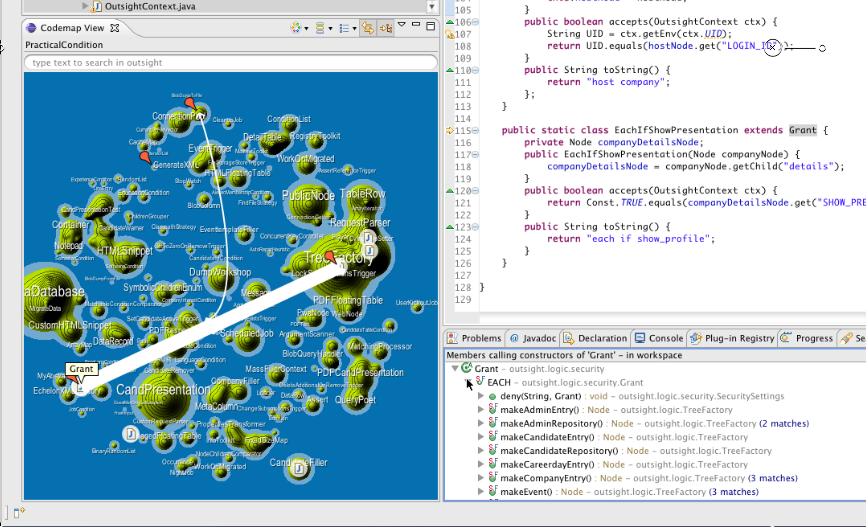
\includegraphics[width=\linewidth]{fig/codemap-userstudy2010-T-fat-arrow-1937}
\end{center}
    \caption{\emph{Screen capture of ``Aha moment'' as encountered by participant~T during task 4-b (location of security features): Upon opening the call hierarchy of \texttt{Grant}'s constructor, a huge call-arrow appeared on the map: indicating dozens of individual calls that connect the security-related archipelago in the south-west with the \texttt{TreeFactory} island in the east. Given the visual evidence of this arrow, participant~T solved the task without further investigation.}}
    \label{fig:fatarrow}
\end{figure}

For this task, participants made most frequent and more interesting use of \Codemap than for any other task. As in task 1, participants used a reversal of the Booch method. They searched for nouns and verbs found in the feature description. Again, they used the map to assess quantity and dispersion of search results. Also two participants used the map to select and inspect search matches based on their context in the map.

Participants now began to read more source code than before. In particular, when they found a promising search result they used the ``open call hierarchy'' feature to locate related classes. All participants reported that \Codemap flow-map overlay helped them to work with the call graph. For some developers there was an actual ``Aha moment'' where one glance at the \Codemap helped them to solve the current subtask immediately without further investigation. \autoref{fig:fatarrow} illustrates one particular moment as encountered by participant~T during the location of the security feature.

\paragraph{Task 5, Code Assesment} This set of tasks made it most obvious that \Codemap's layout was not based on package structure. Participants reported that they had a hard time to interpret the thematic maps as they could not map locations on the map to packages. In particular the professional participants expressed concerns regarding the use of KLOC for hill size. They expressed concerns that this might be misleading since lines of code is not always an indicator of importance or centrality on the system's design.

\paragraph{Task 6, Bug Fixing} Participants mainly used the same approach as for the feature location tasks. They first located the implementation of the feature in which the bug occurs, and then fixed the bug. Professional participants did so successfully, whereas student participants did not manage to find the correct location in the source code.

\paragraph{Wrap-up session} In general, participants reported that \Codemap was most useful when it displayed search results, callers, implementers, and references. A participant reported: \emph{``I found it very helpful that you get a visual cue of quantity and distribution of your search results''}. In fact, we observed that that participants rarely used the map for direct navigation but often for search and reverse engineering tasks.

Another observation was that inexperienced developers (\ie students) are more likely to find the map useful than professional developers. This might be explained by the hypothesis that to power users \emph{any} new way of using the IDE is likely to slow them down, and conversely to beginners \emph{any} way of using the IDE is  novel. The only exception to this observation was \Codemap's search bar, a one-click interface to \eclipse's native search, that was appreciated and used by all participants but one who preferred to use the search dialog.

One participant also provided us feedback comparing his experience with \Codemap to that with the Moose analysis tool \cite{Nier05c}. He uses Moose at work after having attended a tutorial by a consultant. He said he prefers the immediate feedback of Codemap, and reported that \emph{``the gap between Moose and IDE is just too large, not to mention the struggle of importing Java code. Moose helps you to \eg find god-classes but this is typically not new to developers that know a system. Codemap seems more interesting as it integrates with what you actually do in the IDE as you program.''}

\subsection{Observations, Hypotheses, Implications}

In this section, we present an in-depth analysis of our observations, structured by triples of \emph{observation}, \emph{hypothesis}, and \emph{implication}. Implications are directed at improving the design and usability of spatial visualizations that are embedded in an IDE.
% ---- ----- ----- ----- ----- ---- ---
\paragraph{Observation 6.1: When thinking aloud, developers spoke of the system's architecture in spatial terms} 

%\begin{figure}
%\begin{center}
%  \includegraphics[draft,width=\linewidth]{fig/wrapup-map}
%\end{center}
%    \caption{\emph{Spatial map of the system, drawn by one after the participants in the the wrap-up session. All utility packages are located in the upper left corner, separated by a jagged line.}}
%    \label{fig:wrapupmap}
%\end{figure}

The think-aloud protocol revealed that participants refer to the system's architecture in spatial terms. Professional participants referred to packages as being above, below, or at the some level as one another. Some of them even did so before recovering the system's 3-tier architecture in task \#3. Most professionals referred to utility packages a being spatially beside or outside the layered architecture. 

For example, participant~T located all utility packages in the upper left corner, separated by a jagged line. While doing so, he made a gesture as if pushing the utility classes away and stated, \emph{``I am putting them up here because to me they are somehow beside the system.''}

Students on the other hand made much fewer references to the system's architecture, both spatial as well as in general. They were typically reasoning about the system at the level of classes and source lines, rather than in architectural terms. The maps drawn by students in the wrap-up phase, however, showed similar spatial structure to those of the professionals. It remains thus open whether students established a genuine spatial model while working with the code (as we observed for professionals) or only because they were asked to draw the wrap-up maps.

\paragraph{Hypothesis 6.1: Professional developers establish a spatial mental model of the system's architecture}

Based on above observations there is evidence to assume that professional developers establish a spatial mental model of the system's architecture as they work with code. Furthermore, they do so even without visual aids, since they use spatial terms and thinking even before being asked to draw a diagram of the system's architecture.

%\ewe{A few more questions: do devs cluster the things in similar ways, but positions the clusters relatively to one other in a different way? Or is the clustering different among people? Is there a natural tendency to position clusters one way or the other, e.g. UI on the left, Data on the right, Utility at the bottom? If you can say something about that it would be great}

\paragraph{Implication 6.1: Developers should be able to arrange the layout according to their mental model}

This has implications on the design of a system's spatial visualization. Developers should be able to arrange the layout according to their mental model. Developers should be able to drag and move parts of the map around as they wish, rather than having to stick with the automatically established layout. Code Canvas \cite{Deli10a} and Code Bubbles \cite{Brag10b} both already address this implication. In those tools, the user may drag individual elements around and arrange them according to his mental model. 

We observed that developers referred to architectural components, but not classes, in spatial terms. The needs of developers might thus be even better served by providing them more high-level means of arranging the map. Our next prototype will use \emph{anchored multidimensional scaling} such that developers may initialize the map to their mental model. Anchored MDS allows the developer to define anchors which influence the layout of the map \cite[Sec 4.4]{Buja08a}. Any software artifact can be used as an anchor (as long as we can compute a its distance to artifacts on the map), even for example external libraries. In this way, developers might \eg arrange the database layer in the south and the UI layer in the north using the respective libraries as anchors.

\paragraph{Observation 6.2: Participants used Codemap to assess quantity and dispersion of search results and call graphs}

The feature of Codemap that was used most often, by both professionals and students, was the illustration of search results and call graphs. Participants reported that they liked the search-result support of the map, explaining that it gives them much faster initial feedback than Eclipse's tabular presentation of search results. Many participants reported that it was \emph{``as if you could feel the search results,''} and that \emph{``you get an immediate estimate how much was found, whether it is all one place or scattered all over the place.''}

\autoref{fig:fatarrow} illustrates one particular ``Aha moment'' as encountered by participant~T during task 4-b, \ie location of security features: Upon opening the call hierarchy, a huge call-arrow appeared on the map: indicating dozens of individual calls that connect the security-related archipelago in the south-west with the \texttt{TreeFactory} island in the east. Given the visual evidence of this arrow, the participant solved the task immediately without further investigation of the system.

\paragraph{Hypothesis 6.2: Intuitive visualizations to show quantity and dispersion of search results (as well as call graphs) address an important need of developers}

%\ewe{I would maybe generalize it and say: Intuitive visualization to show the quantity and dispersion.... I could imagine that the package explorer could be enriched with a smart way to show search result. E.g. packages with many hits would be red, while packages with few hits would be gray. Or a smart algorithm that would unfold the package to show the relevant class hierarchies. Or something else}

Given the above observation it seems clear that developers have urgent needs for better representation of search results than tabular lists. We found that both students and professionals used the map to get an immediate estimation of search results. This is most interesting since otherwise their use of the tabular search results differed: Professionals glanced at the results, inspected one or maybe two results, and then either accepted or rejected their hypothesis about the system, while students would resort to a linear search through all search results, not daring to reject a hypothesis on the grounds of one or two inspected results only.

Given the map's illustration of search results however, the behavior of both groups changed. Students dared to take quick decisions from a mere glance at the map, whereas professionals were more likely to inspect several results. One professional reported that he \emph{``inspected more results than usual, because the map shows them in their context and that this helps him to take a more informed choice on which results are worth inspection and which ones not.''}

\paragraph{Implication 6.2: Tools should put search results into a meaningful context, so developers can take both quicker and better-informed decisions}

The need for better presentation of search results has implications beyond the design of spatial visualizations. Work on presentation of search results goes beyond spatial maps \cite{Hear09a}, for example results can be presented as a graph. Poshyvanyk and Marcus \cite{Posh07a} have taken one such approach (representing search results as a lattice) and applied it to source code search with promising results. 
%\ewe{Can't agree more}

For our next prototype we plan to integrate search results into the package explorer view, just as is already done with compile errors (which are, from this point of view, just like the search results of a complex query that is run to find syntax errors). This planned feature addresses another implication of our study as well, as we have found that some developers establish a spatial memory of the package explorer view. It therefore makes sense to mark search results both on our map as well as in the explorer view. 
%\ewe{Can't agree more}

\paragraph{Observation 6.3/a: When interacting with the map, participants were attracted to isolated elements, rather than exploring clusters of closely related elements}
 
We found that participants are more likely to inspect easily discernible elements on the map. They are more likely to notice and interact with an isolated island rather than with elements that are part of a larger continent. Unfortunately, it is exactly dense and strongly correlated clusters that contain the most interesting parts of the system! When investigating this issue, participants answered that \emph{``those (isolated) elements looked more important as they visually stick out of the rest of the map.''} 
 
Also, when working with another system that had (unlike the present study) a large cluster in the middle surrounded by archipelagos on the periphery, we found that users started their exploration with isolated hills in the periphery, only then working their way towards the more dense cluster in the middle. 

\paragraph{Hypothesis 6.3/b: Participants rarely used Codemap to return to previously visited locations, instead using package explorer and ``Open Type'' to do so}

Contrary to our assumptions, participants did not use the map to return to previously visited locations by recalling them from spatial memory. Some would use the map, but only for exposed classes that are easily recognizable and clickable. This observation is related to the previous one.

We found however some participants established a spatial memory of the package explorer\,---\,and did so \emph{in addition to their spatial model of the system's architecture!} For example, participant~S would drill down with the explorer saying ``let's open that class down there'' or ``there was this class up here.'' Over the course of the experiment he got quicker at navigating back to previously visited classes in the package explorer. Other participants, as for example participant~T, relied on lexical cues and made extensive use of Eclipse's ``Open Type'' dialog to find their way back to previously visited classes.

Usability glitches will of course worsen the effect of (or might even be the main cause of) not using the map for navigation and revisiting classes. From this it follows that:

\paragraph{Hypothesis 6.3: Developers avoided clusters of closely related elements because they are difficult to identify and select on the map}

All participants had difficulties to open files by clicking on the map. They had difficulties to select classes on the map when they are in a crowded cluster. They would click in the middle of a label, but often the labels are not centered, which is an unavoidable artifact of any labeling algorithm, and thus the clicks would open a different (unlabeled) class.

Codemap does provide tooltips, however participants did not use them. From observing their work it was obvious why: both students and professionals were working at such a speed that waiting for a tooltip to appear would have totally taken them out of their workflow. 

\paragraph{Implication 6.3: The map's layout should be such that all elements are easily discernable and easy to click}

Real estate on a computer screen is limited, and even more so in an IDE with all its views and panels. As tool builders we have limited space available for an embedded visualization. Given our goal of establishing a global layout we face the challenge of having to visualize all elements of a system in that very limited space. 

The current implementation of Codemap has one level of scale only, which may yield crowded clusters where elements are placed just pixels apart. A zoomable map as provided by Code Canvas \cite{Deli10a} addresses this issue. 

The fact that we are attracted by elements that are visually detached has two impacts: one is that we tend to look at isolated elements as being of low significance, the other being that it is hard to identify elements in the cluster. These impacts are very different, but can both be addressed in a common way.
% Both are very different, but might be consolidated.
For instance, a threshold could be used to not show isolated elements at all, but only significant clusters. Alternatively, colors may be used to display isolated elements so that they do not draw our attention so readily.

%\ewe{I'm a bit puzzled with the formulation of 6.3. The fact that we are attracted by elements that visually detach from other has two impacts: (1) one is the we tend to look at isolated element of low significance, the other (2) that it's hard to identify elements in the cluster. Both are very different. The hypothesis  is more related to (1) while hypothesis and implication relates more to (2). The argumentation should be consolidated, IMHO. For instance, a threshold could be used to not show isolated elements at all, but only significant clusters. That would address (1), but not (2). Or the usage of colors, to display isolated element so that they don't attract our look }

\paragraph{Observation 6.4: Participants rarely used Codemap to return to previously visited locations, instead using package explorer and ``Open Type'' to do so}
 
\paragraph{Hypothesis 6.4:  Developers failed to establish a spatial memory of the map not due to its layout but also due to missing visual cues}

In general, the issue of usability is orthogonal to the map's layout. For example, offering ``search as you type'' might help to raise map interaction for those developers that mainly rely on lexical cues, no matter which base layout is used. It was our impression that any exploratory user study of embedded software visualization will be dominated just as by usability issues as by technical factors, such as your choice of layout algorithm. 

\paragraph{Implication 6.4: It should be possible to bookmark classes as ``top landmarks,'' both manually and automatically based on usage statistics}
 
What might help as well to ease the retrieval of previously visited classes is a ``top landmarks'' feature where you can manually (but also automatically based on visits) set markers on the map as starting points for further activities. We plan to work on this for our next prototype. 
%\ewe{The apparent ability to remember position in the package explorer but not in the map may be due to other aspects. I'm wondering for instance if providing a grid in the map with row A-F, and column 0-16 would help to remember the position in the map. Maybe yes, maybe not. In the real-world analogy, maps have latitude and longitude. With never remember them, but help us to slice the map. We maybe need some rigidity to be able to anchor position in our mental model. The package explorer is too rigid, and the map is to flexible/free.} \ewe{All that to say that I don't quite get the link form observation 6.4 to implication 6.4}
%
%\ewe{Actually, I'm wondering if dropping 6.4 altogether wouldn't make the argumentation stronger. To me the main points are 6.1, 6.2, 6.3, 6.5}.

\paragraph{Observation 6.5: Participants used Codemap as if its layout were based on package structure\,---\,even though they were aware of the underlying topic-based layout}

Developers assume that packages are a valid decomposition of the system and expect that the layout of the spatial visualization corresponds to the package structure. We found that clustering classes by topic rather than packages violates the ``principle of least surprise.'' We observed that participants tended to interpret visual distance as a measure of structural dependencies\,---\,even though they were aware of the underlying lexical implementation!
 
Participants expected the layout to reflect at least some structural property. Most of them reacted surprised or confused when for example the classes of a package were not mostly in the same place. For example, Participant~S reported in the wrap-up, \emph{``this is a very useful tool but the layout does not make sense".} Another participant stated during task 3 (\ie the architecture recovery) with confusion that \emph{``the classes contained in packages are scattered on the map, it is not obvious what their spatial connection is.''}
 
\paragraph{Hypothesis 6.5: From the developers view, the predominant mental decomposition of a system is package structure}

Given the general stance of reverse engineering research \cite{Nier05c,Kuhn07a,Duca09c} we had come to distrust package decomposition, however it seems that developers like to rely on the packaging that other developers have made when designing the system.

One problem raised by research in re-packaging legacy systems is that packages play too many roles: as distribution units, as units of namespacing, as  working sets, as topics, as unit of architectural components, etc. However, as an opposing point of view, we can relate packaging to the folksonomies of the Web 2.0, where users label elements with unstructured tags that are then exploited by other users to search for elements. In the same way, we could say that putting trust into a given package structure is a way of collaborative filtering. Developers assume that other developers had made the same choice as they would when packaging the system. 

\paragraph{Implication 6.5: The map layout should be based on code structure rather than latent topics only. However, non-structural data should be used to enrich the layout}

When running the user study, it became quickly apparent that we should revise our initial assumption that lexical similarity is a valid dissimilarity metric for the spatial layout. This was the strongest feedback, and as is often the case in exploratory user studies, already obvious from watching the first professional participant for five minutes only. From all participants we got the feedback that they expect the layout to be structural and that our clustering by topics kept surprising them even after working with the map for almost two hours.
 
Still we think that spatial layouts that go beyond package structure are worthwhile. Therefore, we propose to enrich structure-based layout with non-structural data, such as design flaws. For future work, we are about to refine our layout algorithm based on that conclusion. The new layout is based on both lexical similarity and the ideal structural proximity proposed by the ``Law of Demeter'' (LOD). This is a design guideline that states that each method should only talk to its friends, which are defined as its class's fields, its local variables and its method arguments. Based on this we can defined an {\itshape idealized} call-based distance between software artifacts. Given a LOD-based layout, software artifacts are close to one another if they are supposed to call one another and far apart if they better should not call one another. Thus we get the desired property that visualizing call-graphs conveys meaningful arrow distances. On a LOD-based map, any long-distance-call has a diagnostic interpretation that helps developers to take actions: Long flow-map arrows indicate calls that possibly violate the ``Law of Demeter''.

%\begin{table*}
%\begin{center}
%  \includegraphics[width=\linewidth]{fig/codemap2010-userstudy}
%\end{center}
%    \caption{\emph{Collected data of three selected participants. From top to bottom, categories are: success rate, perceived difficultly, perceived usefulness of the Codemap plug-in, and observed use of IDE features (a single cross indicates use of that feature, and a double cross indicates that the given feature was used the most).}}
%    \label{fig:table}
%\end{table*}

%=========================================================
\section{Threats to Validity}
\label{sec:discussion}

\todo{edit this section}

This section summarizes threats to validity. The study had a small sample size (3 students, 4 professionals) and might thus not be representative. We manually evaluated the data, results might thus be biased. Nevertheless, results are promising and running a pilot think-aloud study with a small user group is a state-of-the-art technique in usability engineering to learn learn about the reactions of users. Such pilot studies are typically used as feedback for further iteration of the tool and to assess the usefulness of its application \cite{Niel03a}.

In this section, we discuss observations regarding the different performance of students and professional participants that are reported in the task performance subsection just below. We found no correlation between codemap interaction and success rates, rather success was completely dominated by the participant's programming experience. Professional participants succeeded in all tasks, where as students failed more than half of all tasks. 
%
Professional developers are very focused, \chg{the} they mainly used keyboard shortcuts only and \chg{goes} go very fast, he seems to ignore not only the map but most parts of the IDE as he goes along, our impression is that he is very focused and always knows exactly where to look next. Professional developers only used a limited set of IDE means to achieve a task, whereas students would typically use all available means (of which they know of, we found that some features where unknown to the students, whereas on the other hand we learned new usages of Eclipse from the professionals. This is a serious challenge for researches, imagine for example that you'd ask your control group to solve a taks in Excel but you are unaware of for example \chg{the} of the Pivot table feature and thus etc).
%
Professional developers would formulate hypotheses first and very quickly and either accepts or rejects them with typically looking at one or two search results only, almost all their conclusions are correct but if they are not they are just as quick to abandon them and move on to the next hypothesis. Where as students, when facing an incorrect hypothesis would stick with it and turn to exhaustive linear search through the system looking for the missing evidence. Similar but not as critical they would often look for more than one prove of a correct hypothesis. \cite{Holm09a}
%
As most researchers in computer science do have a back ground as software engineers, we are often tempted to assume that we proficient software engineers ourselves. Watching the think-aloud footage of the professional participants has though as a better, their use of the IDE showed a proficiency and efficiency that was magnitudes beyond ours and challenged many of our assumptions regarding the use of software maps in an IDE. 
%
It is a known problem to recruit professional participants for user studies, but given our experience with the think-aloud protocol we think it is safe to assume that a study with even few professionals has more predictive power than any study with dozens of students. The needs of seasoned developers are just so different from those of students that still struggling to learn their profession. 
%
One of the most striking difference between students and professionals was that a professional would never do any click or action in the IDE without having a clearly stated hypothesis of what is going on, while students soon turned into repeated ``linear search'' patterns when facing problemens they could not understand. 
%
On the other hand, the students shows a much better adoption rate of the software visualization the the professionals. That was not unexpected, since to power users any new way of using the IDE is likely to slow them down, and conversely to beginners any way of using the IDE is  novel. This raises the question of incremental versus revolutionary improvements: is it possible to prove the usefulness of a revolutionary improvement in a user study? Clearly, for well-defined incremental improvements we can measure the benefit with controlled and repeatable experiments. However, some revolutionary improvements are likely to be rejected by professionals for being not enough in line with their habits but as well as are likely to show no measurable improvement for students, since students are still struggling to learn their profession rather than being able to perform controlled tasks.

% ===================================================================================
\section{Conclusion}
\label{sec:future}

In this paper we presented an evaluation of spatial software visualization in the IDE. We embedded a prototype of the \emph{\SOCA} approach~\cite{Kuhn08a,Erni10a,Kuhn10b}, the \Codemap plug-in, in the Eclipse IDE and ran an exploratory user study which included both students and professionals. 

Software maps are supposed to help developers with a visual representation of their software systems that addresses their spatial thinking and memory. The scenario of our user study was first contact with an unknown closed-source system. Results were as follows:

\begin{itemize}
\item Participants made good use of the map to inspect search results and call graph. They reported that the spatial visualization provided them with an immediate estimate of quantity and dispersion of search results. 
\item Participants found the layout of the map (which uses lexical information to cluster classes by topic) surprising and often confusing. This led to the revision of our initial assumption that lexical similarity is sufficient to lay out the cartographic map.
\end{itemize}

\noindent We drew the following four main observations, and concluded from these the following implications:

\begin{itemize}
\item All participants used a form of spacial thinking to understand the system. It would be best to allow developers to rearrange the initial layout according to their spatial memory.


\item Immediate estimate of quantity and dispersion of search results is useful and the map suits this well. 
\item Participants are distracted by isolated elements, which do not appear in textual/tabular representation. This is the drawback of visualization, which must find the right balance between the power of visualization and the pitfall of visualization. The map should be improved to mitigate that.
\item The coexistence of two models for the software (one structural, one conceptual) causes some confusion. With the present map and implementation, participants were puzzled by non-structural nature of the map.
\end{itemize}

Developers intuitively expect that the map meets their mental model of the system's architecture. We observed that if this is not given, developers are not able to take advantage of the map's consistent layout. So for example, even though north/south and east/west directions had clear (semantic) interpretations in the map used for the user study, developers did not navigate along these axes. 

However, even with the most perfect layout, developers might not be able to take advantage of the map if the elements are barely discernable, and thus difficult to inspect. 

Based on the results of our user study, we conclude with the working hypothesis that \emph{the map should incorporate structural information and be improved from point of usability} and that \emph{we need more work to make two models (one structural, one conceptual) co-exists without creating confusion.} 

%\ewe{Also, I would personally draw another conclusion, which is that Which I think is possible, but requires fine tuning. Devil is in the details! The barrier between "crystal clear" and "plain confused" is maybe not so big. ... But I diverge}

In order to achieve this, we propose the following changes to the \SOCA approach: 

\begin{itemize}
\item Compute the initial layout so that distance reflects structural correlation, since this is what the developers expect (\ie ``principle of least astonishment'').
\item Use \emph{anchored multi-dimensional scaling} for the layout so that developers may rearrange the map according to their spatial model of the system.
\item Use architectural components as anchors for rearrangement of the map, since spatial thinking of developers is strongest at the architectural level.
\item Improve the usability experience of inspecting and selecting of elements on the map, possibly using a zoom\-able user interface.
\end{itemize}

%\ewe{ Software is all about dependencies. The de-facto main view is structural/module dependencies, and the conceptual/feature/topic dependencies are delegated to an auxiliary in-memory map. 
%The question is how should the the 2nd view be displayed.  CodeMap address this problem, but suffers maybe from immaturity. }
%\ewe{Also, given that the topic was not displayed on the map, I'm personally wondering if there isn't a huge bias in the study. Developers don't know the meaning of a cluster: ``Participants reported that they had a hard time to interpret the thematic map''. Looks very legitimate, but very easily to tackle.}
%\ewe{You report that senior dev where confused by the size of the island because KLOC does not reflect the significance of a class, plus the fact that we tend to be attracted to isolated elements. Again, this could be addressed in one way or the other}


